\begin{titlepage}
\vspace*{20mm}
{\Huge\sffamily\bfseries\color{ink}Ecuaciones diferenciales\par}
\vspace{5mm}
{\LARGE problemas, modelos y métodos\par}
\vspace{18mm}
{\Large Giovanni Dalmasso\par}
{\small Departamento de Matemáticas y Analítica de Datos\par}
\vspace{7mm}
{\Large Joaquín Menacho\par}
{\small Departamento de Ingeniería Industrial\par}
\vspace{9mm}
{\normalsize IQS · Universitat Ramon Llull\par}
\vfill
{\large Edición del estudiante\par}
Primera edición · 2026\par
{\small Versión v1.0.0\par}
\end{titlepage}
\chapter*{Créditos y edición}
\thispagestyle{plain}
\textbf{Ecuaciones diferenciales: problemas, modelos y métodos}\par
Giovanni Dalmasso y Joaquín Menacho\par
Edición del estudiante · Versión v1.0.0

© 2026 Giovanni Dalmasso y Joaquín Menacho, por sus aportaciones originales.

Salvo las excepciones expresamente indicadas, el contenido educativo y las figuras originales de esta obra se ofrecen bajo la licencia \href{https://creativecommons.org/licenses/by-sa/4.0/legalcode.es}{Creative Commons Atribución-CompartirIgual 4.0 Internacional (CC BY-SA 4.0)}. La concesión comprende únicamente los derechos que sus titulares están facultados para otorgar.

Las fotografías de los autores se reproducen con autorización y quedan excluidas de la licencia general; no se concede una licencia de reutilización sobre ellas. La ayuda numérica distribuida en \href{https://github.com/gioda/ecuaciones-diferenciales/blob/main/scripts/mallas.py}{\texttt{scripts/mallas.py}} se rige por la licencia MIT que la acompaña.

\textbf{Cubierta.} Imagen generada con inteligencia artificial bajo dirección de los autores. Composición tipográfica realizada por separado. Se licencian los derechos disponibles, sin afirmar exclusividad jurídica sobre la imagen generada.

Las afiliaciones identifican la vinculación académica de los autores y no implican aval institucional.

Las tipografías TeX Gyre Pagella, TeX Gyre Heros, TeX Gyre Pagella Math y Latin Modern Mono empleadas en el PDF conservan su licencia GUST Font License (GFL, basada en LPPL). No se relicencian como contenido propio de la obra. Información y términos: \url{https://ctan.org/license/gfl}. No se distribuyen los paquetes de fuentes por separado.

\textbf{Cita de la obra.} Dalmasso, G. y Menacho, J. (2026).
\emph{Ecuaciones diferenciales: problemas, modelos y métodos}.
Edición del estudiante, v1.0.0.

\textbf{Registro institucional DAU.} [HANDLE DAU PENDIENTE]\par
\textbf{Repositorio y archivos de apoyo.} \url{https://github.com/gioda/ecuaciones-diferenciales}

\textbf{Sobre esta edición.} Libro de problemas para el estudio autónomo de las ecuaciones diferenciales. Reúne 370 ejercicios en diez capítulos, con respuestas de comprobación, nueve pistas y 51 soluciones completas seleccionadas. La modelización y la elección razonada de métodos articulan el recorrido: EDO de primer orden, ecuaciones lineales, oscilaciones, transformada de Laplace y sistemas, seguidos de Fourier, Sturm--Liouville y una introducción a las EDP.

El libro nace de la docencia universitaria de las ecuaciones diferenciales. Los modelos de los ejercicios son idealizaciones didácticas; su uso exige atender a las hipótesis indicadas.
\clearpage
\chapter*{Sobre los autores}\addcontentsline{toc}{chapter}{Sobre los autores}
\noindent\begin{minipage}[t]{.22\textwidth}\vspace{0pt}
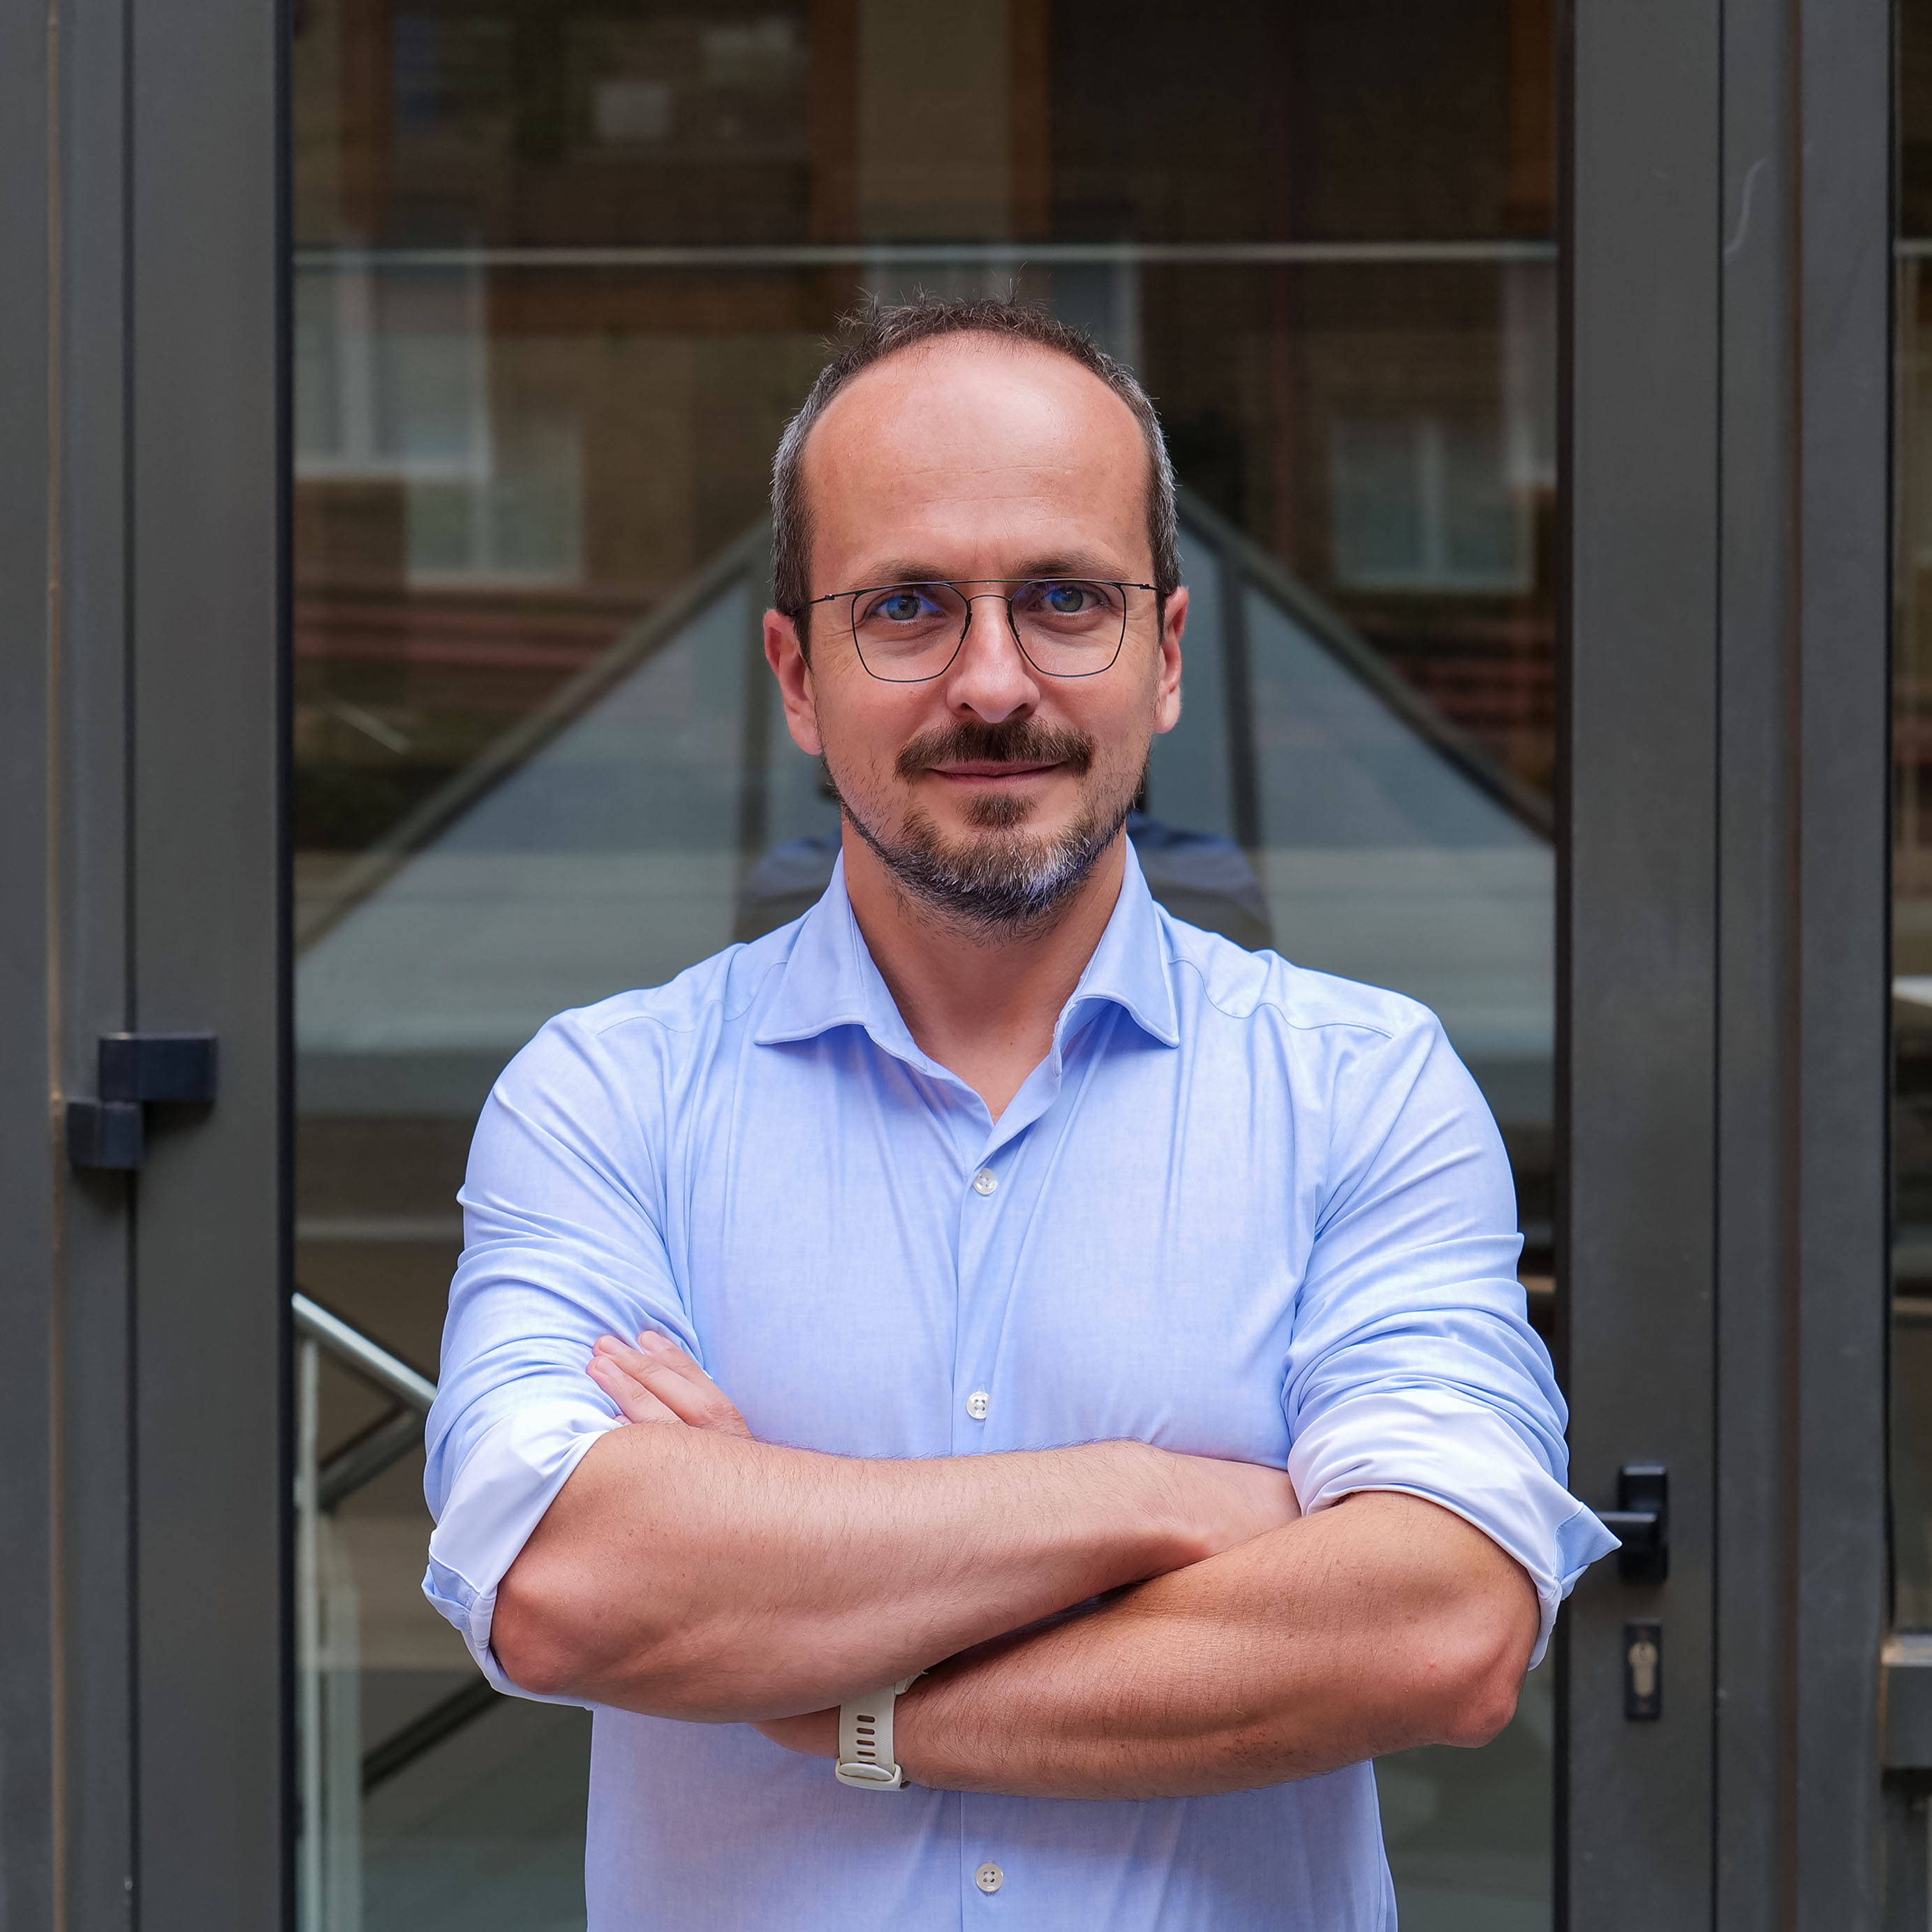
\includegraphics[width=\linewidth,height=40mm,keepaspectratio]{publication_assets/giovanni_dalmasso.jpg}
\end{minipage}\hfill\begin{minipage}[t]{.73\textwidth}\vspace{0pt}
{\Large\sffamily\bfseries\color{ink}Giovanni Dalmasso\par}
{\small\sffamily Departamento de Matemáticas y Analítica de Datos\\IQS · Universitat Ramon Llull\par}
{\footnotesize\href{https://orcid.org/0000-0002-8586-6027}{ORCID: 0000-0002-8586-6027}\par}
\vspace{3mm}Giovanni Dalmasso es ingeniero matemático, formado en el Politecnico di Torino y doctor por la Universidad de Heidelberg (Dr. rer. nat.). Su investigación se sitúa en la intersección de las matemáticas aplicadas, la modelización computacional, la biología y el análisis de datos. En docencia, busca presentar las matemáticas como una disciplina rigurosa, creativa y conectada con problemas reales.
\end{minipage}\par
\vspace{13mm}\par
\noindent\begin{minipage}[t]{.22\textwidth}\vspace{0pt}
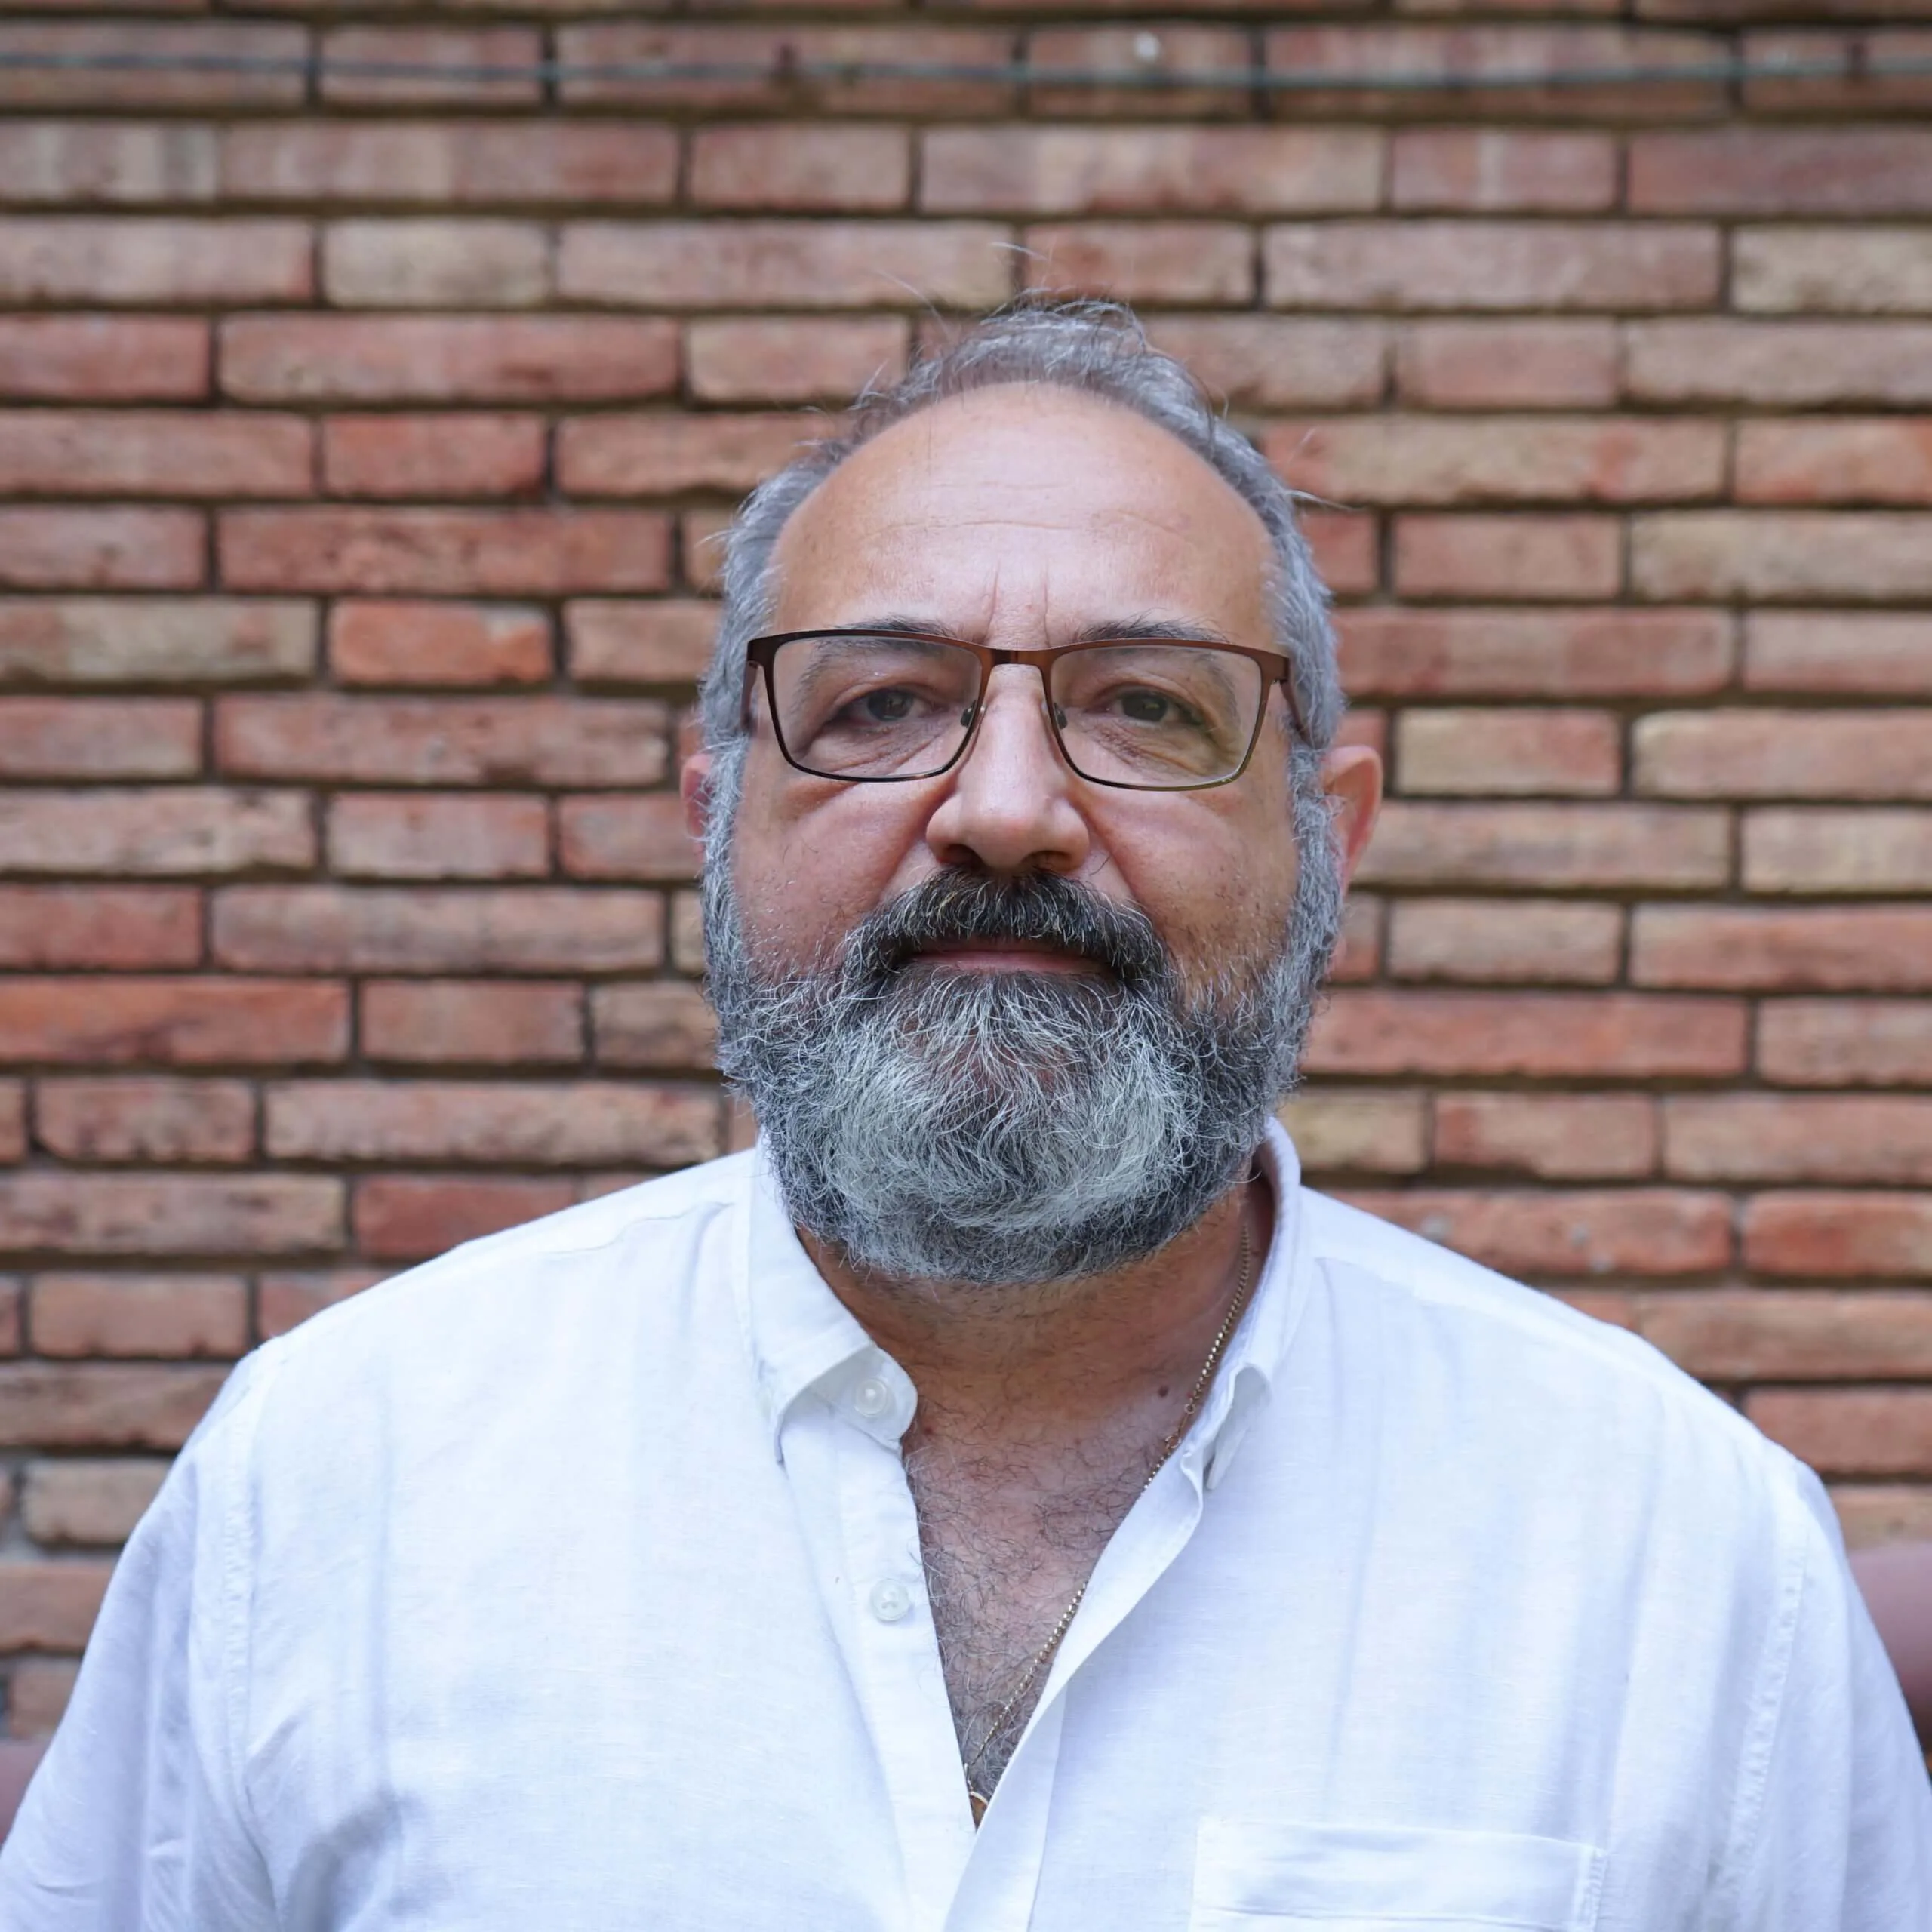
\includegraphics[width=\linewidth,height=40mm,keepaspectratio]{publication_assets/joaquin_menacho.png}
\end{minipage}\hfill\begin{minipage}[t]{.73\textwidth}\vspace{0pt}
{\Large\sffamily\bfseries\color{ink}Joaquín Menacho\par}
{\small\sffamily Departamento de Ingeniería Industrial\\IQS · Universitat Ramon Llull\par}
{\footnotesize\href{https://orcid.org/0000-0001-6895-9021}{ORCID: 0000-0001-6895-9021}\par}
\vspace{3mm}Joaquín Menacho es profesor del Departamento de Ingeniería Industrial de IQS. Es ingeniero industrial por la Universitat Politècnica de Catalunya y doctor en Ingeniería Química por IQS–Universitat Ramon Llull (2012). Su investigación se centra en la modelización matemática, la simulación y la optimización de procesos industriales.
\end{minipage}\par
\clearpage
